\section{Aufbau und Versuchsdurchführung}

Der grundlegende Aufbau bleibt in den einzelnen Versuchsabschnitten gleich, dabei werden teilweise lediglich Geräte hinzugefügt oder getauscht. 
Für die Messung der verschiedenen Moden in Abhängigkeit von der Reflektorspannung $U_{R}$ wird der allgemeinste Aufbau nach Abbildung \ref{fig:1} verwendet.

\begin{figure}
    \centering
    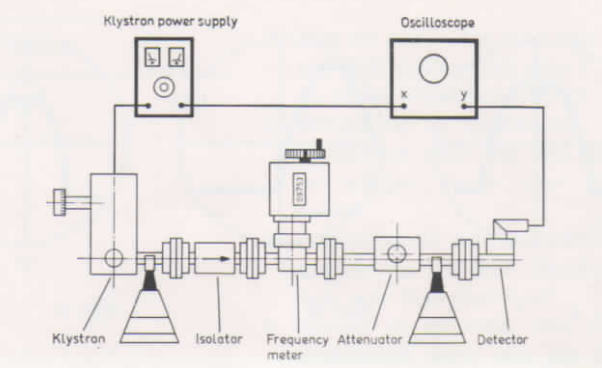
\includegraphics[width=0.6\textwidth]{bilder/grundaufbau.png}
    \caption{Grundlegender Aufbau zur Untersuchung von Mikrowellenstrahlung. \cite{skript}} 
    \label{fig:1}
\end{figure}
Zu sehen ist zunächst das Reflexklystron welches an ein Netzteil angeschlossen ist. Die durch das Klystron erzeugten Mikrowellen werden über einen Hohlleiter aus dem Resonator ausgekoppelt und durch einen Einweggleichrichter geführt. 
Dieser dient dazu, dass keine Mikrowellen in das Klystron zurückreflektiert werden und somit für Ungenauigkeiten sorgen. 
Dahinter werden sowohl Frequenzmessgerät, als auch eine Dämpfungsquelle geschaltet. Die Messung geschieht über einen Detektor welcher mit einem digitalen Oszilloskop verbunden wird. 
Über den gesamten Versuchszeitraum wird die Kathodenspannung konstant bei $U_{K} = \SI{6.3}{\volt}$ belassen.

\subsection{Messung der einzelnen Moden}

Um die Moden der durch den Klystron erzeugten Mikrowellen zu messen wird eine konstante Dämpfung von $\SI{30}{\decibel}$ am Dämpfungsglied eingestellt. 
Dabei lässt sich die angebrachte Dämpfungskurve verwenden. Ein Channel des Oszilloskop wird nun
über ein BNC-Kabel am \enquote{$\SI{0}{}$-$\SI{30}{\volt}$, $\SI{50}{\hertz}$ $\sim$} Ausgang des Netzteils angeschlossen. Ein zweiter Channel wird mit dem Detektor wie in Abbildung \ref{fig:1}
erkennbar verbunden. Es lässt sich ein $x$-$y$ Diagramm von der am Netzteil einstellbaren Reflektorspannung $U_R$ und der Mikrowellenamplitude $U_D$ anzeigen. Das Oszilloskop wird so konfiguriert, dass die ganzen Peaks erkennbar 
und die Amplitude leicht ablesbar ist. 
\\
\newline
Nun lässt sich die erste Mode bei einer Reflektorspannung von $U_R$ \approx $\SI{200}{\volt}$ finden. Dieser Peak wird auf dem Oszilloskop zentriert und somit lässt sich die Reflektorspannung $U_R$ des Peaks bei genau diesem Punkt angeben.
Sobald der Peak gefunden wurde, kann mit dem Frequenzmesser die Frequenz bestimmt werden. Dabei wird solange am Messgerät gedreht bis ein Dip in dem Peak der Mode entsteht. Dieser Messwert beschreibt nun also die Frequenz der Mode.
Der Vorgang wird ebenfalls für die Ränder der Peaks gemacht und anschließend für zwei weitere Moden wiederholt.
\\
\subsection{Messung der Frequenz und Wellenlänge im Halbleiter}
Um die Frequenz der Mikrowelle im Halbleiter zu messen, wird ein SWR-meter verwendet, dazu wird der Aufbau wie in Abbildung \ref{fig:2} erkennbar angepasst. Hinter dem Dämpfungsglied wird eine weitere Sonde eingebaut welche direkt mit dem SWR-meter über
ein BNC-Kabel verbunden ist.

\begin{figure}
    \centering
    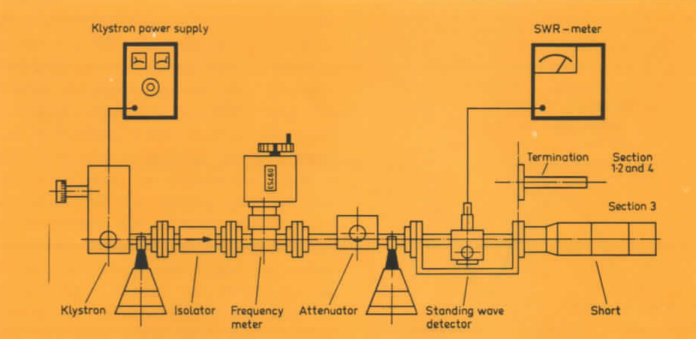
\includegraphics[width=0.9\textwidth]{bilder/aufbau2.png}
    \caption{Aufbau zur Bestimmung der Frequenz, Wellenlänge und Dämpfung. \cite{skript}} 
    \label{fig:2}
\end{figure}
Die Dämpfung wird nun auf $\SI{20}{\decibel}$ eingestellt und am SWR-meter wird die Dämpfung auf $\SI{40}{\decibel}$ angepasst. Da die Detektorsonde keine Frequenzen im Gigahertzbereich detektieren kann wird das Signal mit einer $\SI{1}{\kilo\hertz}$ Rechteckspannung
moduliert. Mit der verschiebbaren Sonde wird nun eine Stelle gesucht bei der am SWR-meter ein Maximum erkennbar ist. An dieser Stelle wäre jetzt am Oszilloskop ein Wellenberg erkennbar und die Frequenz lässt sich wieder über den Frequenzmesser
durch Verschiebung des Dips, bishin zum Minimum am SWR-meter, bestimmen.
\\
\newline
Für die Bestimmung der Wellenlänge genügt in der Theorie auch die Frequenz, dafür muss allerdings die Dispersion bekannt sein. Um die Wellenlänge im Hohlleiter dennoch auch ohne bekannte Dispersion
experimentell bestimmen zu können, wird das Prinzip der stehenden Wellen ausgenutzt. Am Ende des Aufbaus wird der Mikrowellenabschluss mit einem Kurzschluss gewechselt. In dem Hohlleiter bildet sich nun eine stehende Welle
und die Wellenlänge lässt sich so genauer bestimmen.
Die Sonde wird dazu so verschoben, dass ein Minimum oder Maximum am SWR-meter zu erkennen ist. Anschließend wird das daneben liegende Extremum gleicher Art gesucht. Beide Positionen der Sonde werden notiert.

\subsection{Dämpfungsmessung}
Für die Messung der Dämpfung des eingebauten Dämpfungsglieds wird der Kurzschluss wieder mit dem Abschluss getauscht. Zunächst wird die Schraube komplett herausgedreht, sodass in der Theorie, keine Dämpfung stattfindet. Das SWR-meter wird auf 
$\SI{30}{\decibel}$ eingestellt und
so konfiguriert, dass eine Dämpfung von Null angezeigt wird. In $\SI{2}{\decibel}$ Schritten wird nun bis $\SI{10}{\decibel}$ die Mikrometereinstellung des Dämpfungsglieds notiert.

\subsection{Stehwellenverhältnismessung}
In dem Versuch werden drei verschiedene Methoden zur Bestimmung des Stehwellenverhältnis von Mikrowellen in Hohlleitern untersucht.

\subsubsection{Direkte Methode}
Um das Stehwellenverhältnis zu messen liegt eine Methode nach den vorherigen Durchführungen nahe. Das verwendete SWR-meter lässt sich direkt zur Messung des Stehwellenverhältnisses nutzen. Der Aufbau wird um ein Gleitschraubentransformator erweitert
und der Kurzschluss mit dem Abschluss getauscht. Dieser Aufbau ist in Abbildung \ref{fig:3} zu erkennen. 

\begin{figure}
    \centering
    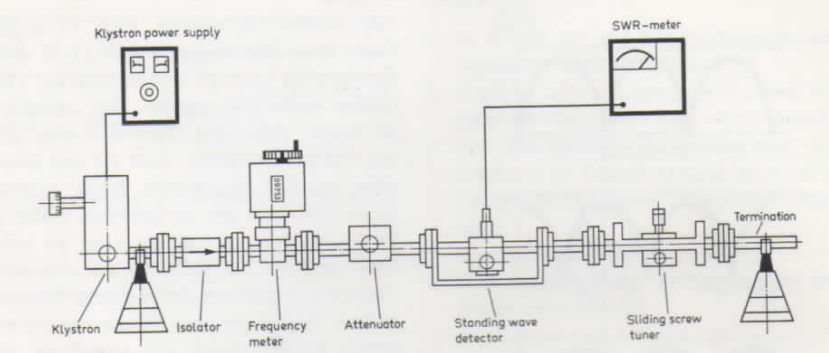
\includegraphics[width=0.9\textwidth]{bilder/aufbau3.png}
    \caption{Aufbau zur Bestimmung des Stehwellenverhältnisses. \cite{skript}} 
    \label{fig:3}
\end{figure}
Der Abschwächer wird wieder auf $\SI{20}{\decibel}$ und das SWR-meter auf $\SI{40}{\decibel}$ eingestellt. Der Gleitschraubentransformator wird zunächst komplett herausgedreht und die Reflektorspannung wieder mit $\SI{1}{\kilo\hertz}$ moduliert.
Da in der Theorie keine Reflektionen auftreten sollten, zeigt die Messsonde nurnoch kleine Änderungen des SWR-Werts bei Verschiebung der Sonde. Durch die eingebauten Geräte kommt es dennoch bereits zu Reflexionsmöglichkeiten, somit muss 
der SWR-meter in diesem Zustand auf ein Stehwellenverhältnis von $\SI{1.0}{}$ kalibriert werden. Nun wird mit ansteigender Gleitschraubentiefe in $\SI{2}{\milli\meter}$ Abständen der SWR-Wert notiert.

\subsubsection{3 dB-Methode}
Für diese Messmethode wird der Gleitschraubentransformator auf $\SI{9}{\milli\meter}$ gestellt und die Sonde so verschoben, dass ein Minimum am SWR-meter angezeigt wird und die Verstärkung auf $\SI{3}{\decibel}$ kalibriert.  Dies hat zufolge, dass 
sobald die Verstärkung auf $\SI{0}{\decibel}$ steht eine doppelte Leistung gemessen wird. Die beiden Stellen, links und rechts, neben diesem Minimum werden abgefahren und die Distanz notiert. Da für die Berechnung auch die
Wellenlänge der Mikrowelle wichtig ist, wird hier nochmal die Wellenlänge über die Abstände zweier Minima berechnet. Diese Stellen werden also ebenfalls festgehalten.

\subsubsection{Abschwächermethode}
Bei der Abschwächermethode bleiben die vorherigen Einstellungen der Geräte beibehalten und der Gleitschraubentransformator auf $\SI{9}{\milli\meter}$ belassen. Gesucht sind die einstellbaren Abschwächungen des Dämpfungsglieds bei denen der SWR-meter 
ein gleiches Stehwellenverhältnis bei relativen Maximum und Minimum besitzt. Diese Differenz gibt also die Verstärkung der gemessenen Leistung an und kann somit auf das Stehwellenverhältnis zurückgeführt werden.
Mit der Sonde wird ein Minimum abgefahren und das SWR-meter so eingestellt, dass eine Verstärkung von $\SI{3}{\decibel}$ angezeigt wird. Die eingestellte Dämpfung wird notiert und anschließend wird das relative Maximum über die Sonde gefunden. Die Dämpfung wird solange
geändert bis wieder eine $\SI{3}{\decibel}$ Verstärkung zu sehen ist.

